\documentclass[11pt]{beamer}
\usetheme{Madrid}
\usepackage[utf8]{inputenc}

\usepackage[brazil]{babel}

\usepackage{amsmath}
\usepackage{amsfonts}
\usepackage{amssymb}
\usepackage{graphicx}
\DeclareMathOperator {\argmin}{argmin}

\author{Autor}
\title{Título da apresentação}
% Informe o seu email de contato no comando a seguir
% Por exemplo, alcebiades.col@ufes.br
\newcommand{\email}{email}
%\setbeamercovered{transparent} 
\setbeamertemplate{navigation symbols}{} 

\institute[]{UNIVERSIDADE FEDERAL DO ESPÍRITO SANTO \par MESTRADO PROFISSIONAL EM MATEMÁTICA EM REDE NACIONAL} 
\date{\today} 
%\subject{}

% ---------------------------------------------------------
% Selecione um estilo de referência
\bibliographystyle{apalike}

%\bibliographystyle{abbrv}
%\setbeamertemplate{bibliography item}{\insertbiblabel}
% ---------------------------------------------------------

% ---------------------------------------------------------
% Incluir os slides nos quais as referências foram citadas
%\usepackage[brazilian,hyperpageref]{backref}

%\renewcommand{\backrefpagesname}{Citado na(s) página(s):~}
%\renewcommand{\backref}{}
%\renewcommand*{\backrefalt}[4]{
%	\ifcase #1 %
%		Nenhuma citação no texto.%
%	\or
%		Citado na página #2.%
%	\else
%		Citado #1 vezes nas páginas #2.%
%	\fi}%
% ---------------------------------------------------------

\begin{document}

\begin{frame}
\titlepage
\end{frame}

\begin{frame}{Sumário}
\tableofcontents 
\end{frame}

\section{Uvod}

\begin{frame}{Introdução}
 Texto referente à introdução.
\end{frame}

\section{Modeli automobila}

\begin{frame}{Modeli automobila koji su obeležili 2022. godinu}{\thesection \, \secname}

\begin{itemize}
\item Problemi sa Covid-19 
\item Ugradnja uredaja za "inteligentno podešavanje brzine"
\end{itemize}
\end{frame}

\begin{frame}{Modeli automobila koji su obeležili 2022. godinu}
Neki od modela koje su predstavile poznate auto kuće su:
\begin{itemize}
\item Škoda Enyaq iV
\item Renault Austral
\item Mercedes-Benz Vision EQXX
\item Evolute i-Pro
\item Drako Dragon

\begin{figure}[h]
        \centering
        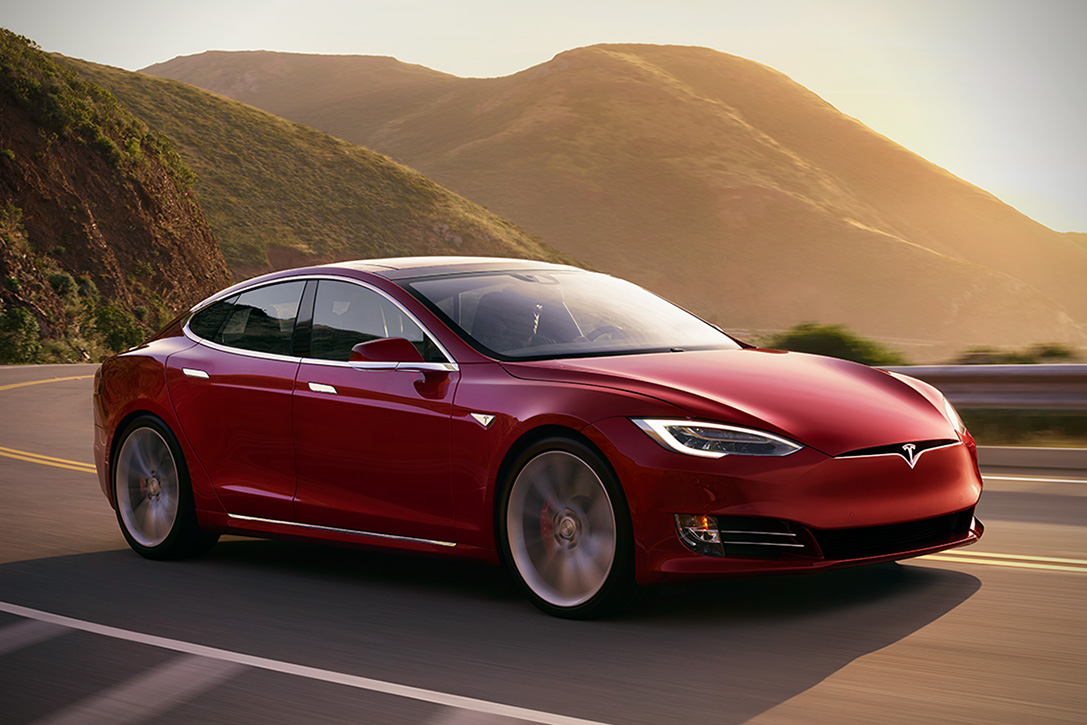
\includegraphics[width=60mm, scale=0.5]{tesla.jpeg}
        \label{fig:tesla.jpeg}
        \end{figure}

\end{itemize}

\end{frame}

\begin{frame}{Listas}
    Exemplo de lista com símbolos:

    \begin{itemize}
        \item Primeiro elemento
        \item Segundo elemento
    \end{itemize}
    
    \bigskip
    
    Exemplo de lista com itens enumerados:
    
    \begin{enumerate}
        \item Primeiro elemento
        \item Segundo elemento
    \end{enumerate}
\end{frame}

\begin{frame}{Tabelas}
    A Tabela mostra um modelo de tabela.

    \begin{table}[htb]
        \caption{Exemplo de tabela}
        \label{tab:modelo_tabela}
        \centering
        \begin{tabular}{c|c|c|c}
	        \hline
	        \textbf{Pessoa} & \textbf{Idade} & \textbf{Peso} & \textbf{Altura} \\ \hline
	        Marcos & 26    & 68   & 178    \\ \hline
	        Ivone  & 22    & 57   & 162    \\ \hline
	        Sueli  & 40    & 65   & 153    \\ \hline
        \end{tabular}
        
        \medskip
        
        Fonte: Produção do próprio autor.
    \end{table}
\end{frame}

\begin{frame}{Imagens}
    A Figura mostra a logomarca promocional da Universidade Federal do Espírito Santo (UFES).
    
    \begin{figure}[htb]
      
        
        \medskip
        
        Fonte: Produção do próprio autor.
    \end{figure}
\end{frame}

\begin{frame}{Conclusão}
    Texto referente à conclusão.
\end{frame}

\begin{frame}{Trabalhos futuros}
    \begin{itemize}
        \item Estudar $\ldots$
        
        \medskip
        
        \item Explorar $\ldots$
        
        \medskip
        
        \item Analisar $\ldots$
    \end{itemize}
\end{frame}

\section{Referências}
\begin{frame}{Referências}
    \bibliography{referencias}
\end{frame}

\begin{frame}

\begin{center}
    Obrigado!
    
    \email
\end{center}

\begin{figure}[htb]
    \centering

\end{figure}

\end{frame}

\end{document}
